\subsection{Modelo E/R propuesto del catálogo}
\label{sec:catalogo-er}
\textit{Diagrama: Alexander. Validación del catálogo desplegado: coordinación con Fabricio.}

El modelo documenta 19 tablas lógicas procedentes de tres fuentes operacionales:
seis de MS1 (MySQL), ocho de MS2 (PostgreSQL) y cinco de MS3 (MongoDB aplanado).
Se plantea como referencia para el catálogo \texttt{aeropuerto\_lake} y los
JOIN de Athena. Su entrega no demuestra que las 19 tablas estén creadas en Glue;
los nombres y tipos finales deben contrastarse con la salida real de ingesta.

\begin{table}[htbp]
\centering\small
\begin{tabularx}{\textwidth}{p{0.10\textwidth}p{0.17\textwidth}X}
\toprule Fuente & Prefijo S3 previsto & Tablas del modelo \\
\midrule
MS1 (6) & \path{raw/ms1/} & persona, categoria\_migratoria, pasajero, ticket, equipaje, checkin. \\
MS2 (8) & \path{raw/ms2/} & aerolinea, aeronave, vuelo, empleado, asiento, tripulacion, operativo\_tierra, opera\_tripulacion. \\
MS3 (5) & \path{raw/ms3/} & recurso, incidencia, incidencia\_afecta\_recurso, incidencia\_retrasa\_vuelo, asignacion. \\
\bottomrule
\end{tabularx}
\caption{Distribución de las 19 tablas del catálogo propuesto.}
\end{table}

MS4 no agrega una fuente persistente al catálogo: consolida respuestas de otros
servicios sin base de datos propia. MS5 consume las consultas de Athena,
por lo que tampoco constituye una cuarta fuente operacional.

Las líneas continuas representan asociaciones lógicas dentro de cada origen.
Las líneas naranjas discontinuas identifican relaciones entre fuentes. Las marcas
PK/FK describen claves del modelo de origen o claves lógicas de unión; no
representan restricciones de integridad ejecutadas por Glue. Los signos de
interrogación señalan atributos opcionales y las estrellas destacan entidades
de negocio.

\begin{table}[htbp]
\centering\small
\begin{tabularx}{\textwidth}{X X}
\toprule Campo de referencia & Clave de unión \\
\midrule
\path{ticket.id_vuelo} (MS1) & \path{vuelo.id} (MS2) \\
\path{equipaje.id_vuelo} (MS1) & \path{vuelo.id} (MS2) \\
\path{asignacion.id_vuelo} (MS3) & \path{vuelo.id} (MS2) \\
\path{incidencia_retrasa_vuelo.id_vuelo} (MS3) & \path{vuelo.id} (MS2) \\
\bottomrule
\end{tabularx}
\caption{Referencias suaves que permiten relacionar las fuentes.}
\end{table}

En MS1, persona y pasajero comparten identificador; tickets y equipajes
se relacionan con el pasajero y checkin con el ticket.
En MS2, vuelo referencia aerolínea y aeronave; la tabla
\texttt{opera\_tripulacion} representa la asociación entre vuelos y tripulantes.
En MS3, el aplanamiento separa los vínculos de incidencias con recursos y vuelos,
permitiendo consultar esas relaciones con JOIN.

Antes de presentar el modelo como catálogo implementado deben verificarse
nombres, tipos, nulabilidad, duplicados en claves y referencias sin correspondencia.
Las diferencias se corrigen de acuerdo con los archivos de ingesta y el catálogo
efectivo, incluyendo los nombres de las tablas de asociación de MS3.
\pendiente{Contrastar el diagrama con Glue y los archivos S3; registrar la fecha
de esa revisión y la evidencia de las consultas de validación.}

\clearpage
\begin{figure}[p]
\centering
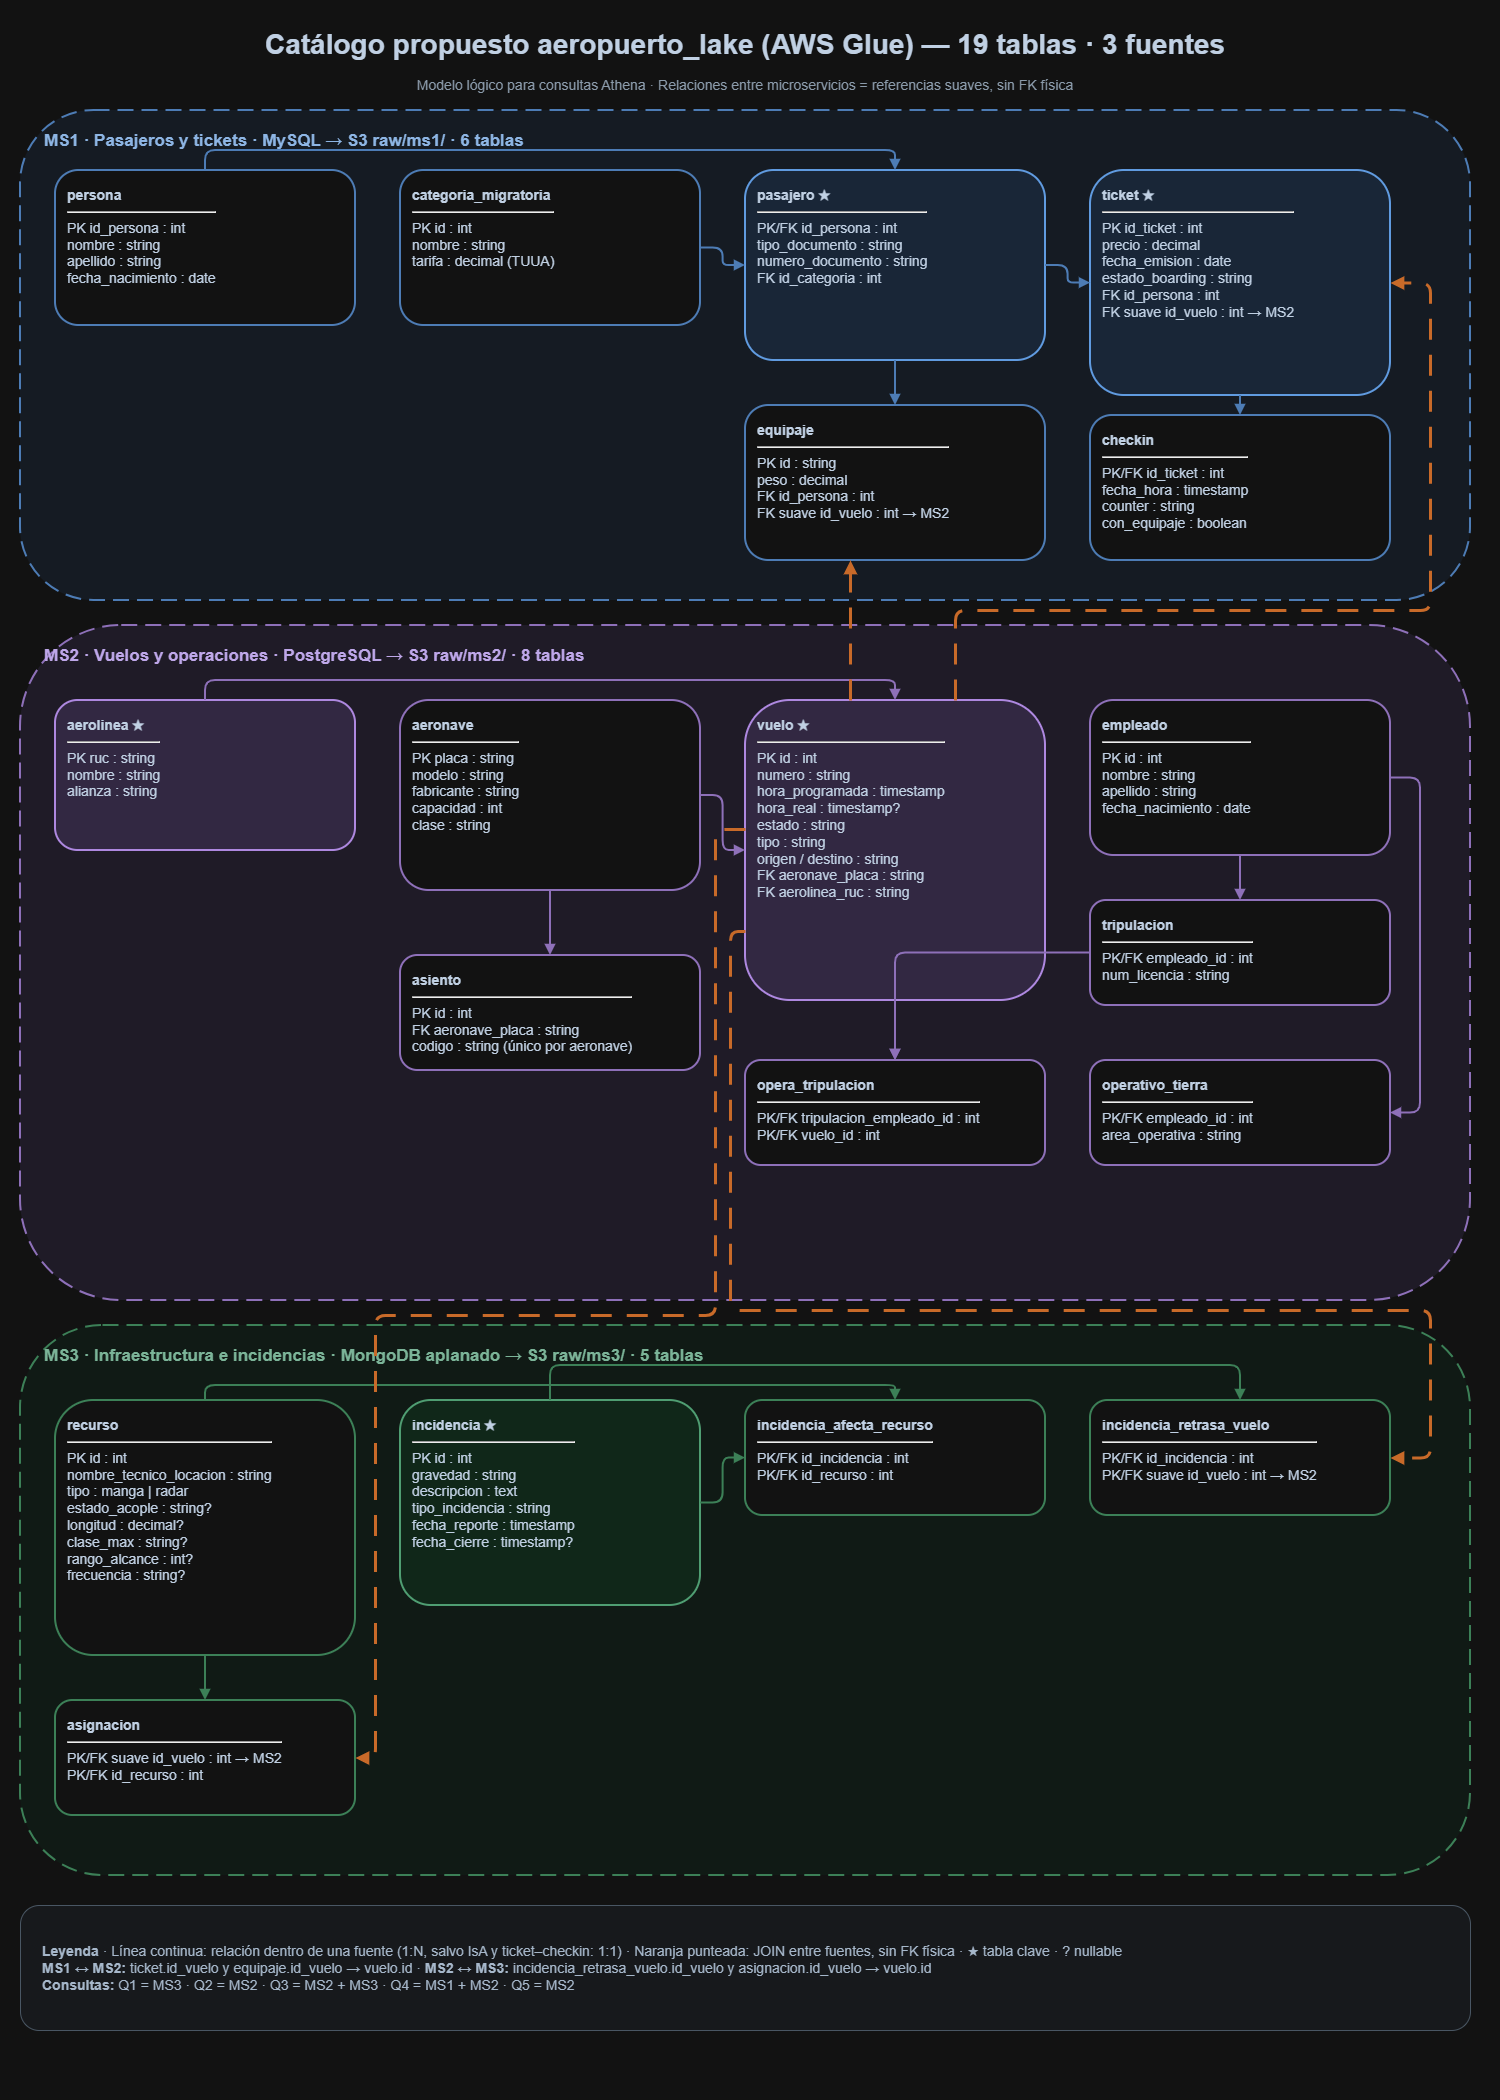
\includegraphics[width=\linewidth,height=0.86\textheight,keepaspectratio]{imagenes/er-catalogo-datalake.png}
\caption{Modelo E/R propuesto del catálogo, 19 tablas y tres fuentes (E-6.4).
Fuente editable: \texttt{diagramas/er-catalogo-datalake.drawio}.}
\label{fig:er-catalogo}
\end{figure}
\clearpage
